\documentclass[./thesis.tex]{subfiles}

 
\begin{document}

\label{chap:exp_dressing}

While CI methods are common ways to account for electron correlation, they suffer a severe size consistency problem.


The logics of the electronic Many-Body problem has been clarified a long time
ago in the situations where  the  wave  function  may  be  generated  from  a
single  determinant  (or  single  reference).  Perturbative  developments,
translated  in  terms  of  diagrams,  led  to  the  formulation  of  the
fundamental  linked  cluster  theorem,\cite{Goldstone}  and  clarified  the  defects  of
truncated  Configuration Interaction  methods.  The  conditions  for  a  good
scaling  of  the  correlation  energy  and  for  the  strict separability  into
closed  shell  fragments  were  established.

By  strict  separability  (which
is  less ambiguous than the terms size-extensivity and size consistency) we
mean that at the non-interacting limit of an $A\cdots B$ problem the energies are
additive, $E_{AB} = E_A+E_B$, and that the amplitudes associated with the single
and  double excitation operators  are  the  same  as  those  obtained  for  the  isolated  $A$
and  $B$  problems.  
Why this is not the case in CI methods can be easily understood as the absence of some excitations occurring simultaneously on all subsystems.

Consider a supersystem $AB$ made of two non-interacting subsystems $A$ and $B$, and write its CID wavefunction (Hartree-Fock determinant and all its double excitations).
\begin{equation}
\Psi^{AB} = \Psi_{\HF}^{AB} + \Psi_{D}^{AB}
\end{equation}
with $\Psi_{\HF}^{AB}$ the Hartree-Fock determinant for system $AB$, and $\Psi_{D}^{AB}$ the sum of all double excitation with respect to $\Psi_{\HF}^{AB}$.

If we now write $\Psi^{A\cdots B}$ the product of the two separate CID wavefunctions for $A$ and $B$
\begin{align}
\Psi^{A\cdots B} = & \Psi^A  \times \Psi^B \\
 = & \Psi_{\HF}^A\Psi_{\HF}^B  + \Psi_{\HF}^A\Psi_{D}^B + \Psi_{D}^A\Psi_{\HF}^B + \Psi_{D}^A \Psi_{D}^B 
\end{align}
As can be seen, $\Psi^{AB}$ isn't described as the product of $\Psi^A$ and $\Psi^B$ as it should, since simultaneous double excitations on $A$ and $B$ cannot be accounted for.

%\begin{equation}
%\Psi^{A\cdotsB} - \Psi^{AB}  = \Psi_{D}^A \Psi_{D}^B
%\end{equation}

Some methods aim at partially or fully correcting this size-consistency error by eliminating the unlinked effects of the CISD: the so-called \emph{Davidson corrections}, that are essentially correction to the energy\cite{Langhoff_1974,Meissner_1988}, and the so-called \emph{Coupled Electron Pair Approximations (CEPA)} that correct the CI equations\cite{Kelly_1963,Kelly_1964,Meyer_1971,Meyer_1973,Meyer_1974,Ahlrichs_1975}. Many different variations have been proposed, for a review see~\citep{Koch_1981}.

An alternative to CI approaches is the so-called Coupled-Cluster (CC) approach, that does not suffer this problem. The wavefunction is given an exponential structure
\begin{equation}
\ket \Psi = e^{\hat T} \ket {\HF}
\end{equation}
with $\hat T$ a so-called \emph{cluster operator}. In the widely used \emph {Coupled Cluster Single and Double (CCSD)} method, the cluster operators is
\begin{equation}
\hat T = \hat T_1 + \hat T_2
\end{equation}
with $\hat T_1$ and $\hat T_2$ the one and two orbitals cluster operators 
\begin{align}
\hat T_1 = \sum_{pr} t_p^r \hat T_p^r \\
\hat T_2 = \sum_{pqrs} t_{pq}^{rs} \hat T_{pq}^{rs}
\end{align}
with the indices $p,q$ running on occupied MOs and $r,s$ running on virtual MOs. $\hat T_{pq}^{rs}$ is the usual excitation operator, and $t_{pq}^{rs}$ the so-called \emph{amplitude} associated with it.

Again considering a system made of two infinitely non-interacting sub-systems $A$ and $B$, thanks to the exponential expression, if one uses local orbitals ---~that is, the reference determinant $\ket {\HF}$ is factorizable in $\ket{\HF_A}$ and $\ket{\HF_B}$ determinants isolated on $A$ and $B$~--- the energy and wavefunction on the isolated fragments will be the same as on the $A\cdots B$ supersystem.
Indeed, amplitudes associated with excitations involving orbitals for both fragments will be zero due to the absence of interaction. Therefore $\hat T$ can be split in $\hat T_A$ and $\hat T_B$ the cluster operators involving one fragment.
\begin{equation}
\ket \Psi = e^{\hat T} \ket {\HF} = \ket \Psi = e^{\hat T_A + \hat T_B} \ket {\HF} = e^{\hat T_A} \ket {\HF_A} e^{\hat T_B} \ket {\HF_B}
\end{equation}
The wavefunction of the supersystem is the product of the wavefunctions for the isolated subsystems.


In the article presented in section~\ref{sec:exp_article}, we have proposed a definition for amplitudes for coupled cluster in a multi-reference context. The somewhat ``brute force'' initial implementation of our \emph{Multi-Reference Coupled Cluster} (MR-CC) was re-written as a stochastic matrix dressing, based on our Shifted-\Bk implementation.

\section{Computing $c_\alpha$}
Whether the matrix dressing algorithm performs a Shifted-\Bk, an MR-CCSD or some other method, depends on the external space, i.e. the $c_\alpha$ coefficients. Our goal is to set up a framework in which stochastic matrix dressing can be done efficiently using an external space only defined by $Z(\alpha, \Psi, \ldots)$ a function that takes a determinant $\kalpha$ and the wavefunction $\ket \Psi$, and returns the $c_\alpha$ it should be associated with. The ``$\ldots$'' notation indicates that the returned value may depend on any number of global parameters, such as approximation thresholds, etc\dots

Looking at the expression of $c_\alpha$ for Shifted-\Bk, it looks like the computation required is the exact same as the one performed by our CIPSI
\begin{equation}
c_\alpha = \frac{\Hij{\alpha}{\Psi}}{\Delta E_\alpha} = \sum_{I=1}^{\Ndet} c_I \frac{\Hij{\alpha}{D_I}}{\Delta E_\alpha},
\end{equation}
but the expression of $c_\alpha$ for Shifted-\Bk has a particularity that lifts a constraint compared to the general case: as can be seen, while for any $\kalpha$ we need to find all internal determinants it connects to, we do not need to know them \emph{at the same time}, i.e. $c_\alpha$ can be incrementally built from terms that only involve one internal determinant at a time. This is not generally the case, and isn't the case in MR-CC.

Thus, matrix dressing generally requires the knowledge of all internal determinants a particular $\kalpha$ connects to, before $c_\alpha$ ---~and thus the associated increment to $\deltabold$~--- can be computed. For efficiency, as well as simplicity, this list must absolutely be computed upstream the computation of $Z(\alpha, \Psi, \ldots)$, making it in practice $Z^\star(\alpha, \Psi_{c}, \ldots)$ with $\Psi_{c}$ the variational wavefunction stripped of all determinants that do not connect to $\kalpha$ (thus not normalized). In practice, it is a list of internal determinant indices.

This is a lot like the former implementation of CIPSI : considering one $\kalpha$ at a time, enumerate its connections to selectors. The new, more efficient algorithm, however, considers a batch of up to $\Nvirt = \qty(\Norb - \Nalpha)^2$ rather than a single one. The solution is conceptually simple. Neglecting connections to determinants that are not selectors :
\begin{enumerate}
\item
Loop over all $G_{pq}$ batches in the same way as in the CIPSI algorithm (building the $B_{rs}$ tag matrix).
\item
For each batch, create ${(2 \Norb)}^2$ sets of internal determinant indices $\mathcal{C}_{rs}$, each associated with $\Gpqrs$.
\item
When a connection between a selector $\ket {D_I}$ and $\kalpha = \ket {G_{pq}^{rs}}$ is found, add $I$ to $\mathcal{C}_{rs}$ (instead of incrementing $P(G_{pq})$).
\item
When the computation of batch $G_{pq}$ is completed, $\mathcal{C}_{rs}$ is the set of all indices of selectors connected to $\kalpha = \ket {G_{pq}^{rs}}$. For each untagged $\kalpha$:
\begin{enumerate}
\item
$c_\alpha \gets Z^\star(\alpha, \mathcal{C}_{rs}, \ldots)$.
\item
For each index $K \in \mathcal{C}_{rs}$ increment $\delta_K$ with $c_\alpha \Hij{\alpha}{S}$.
\end{enumerate}


\end{enumerate}


\begin{figure}[h!]
	\begin{center}
		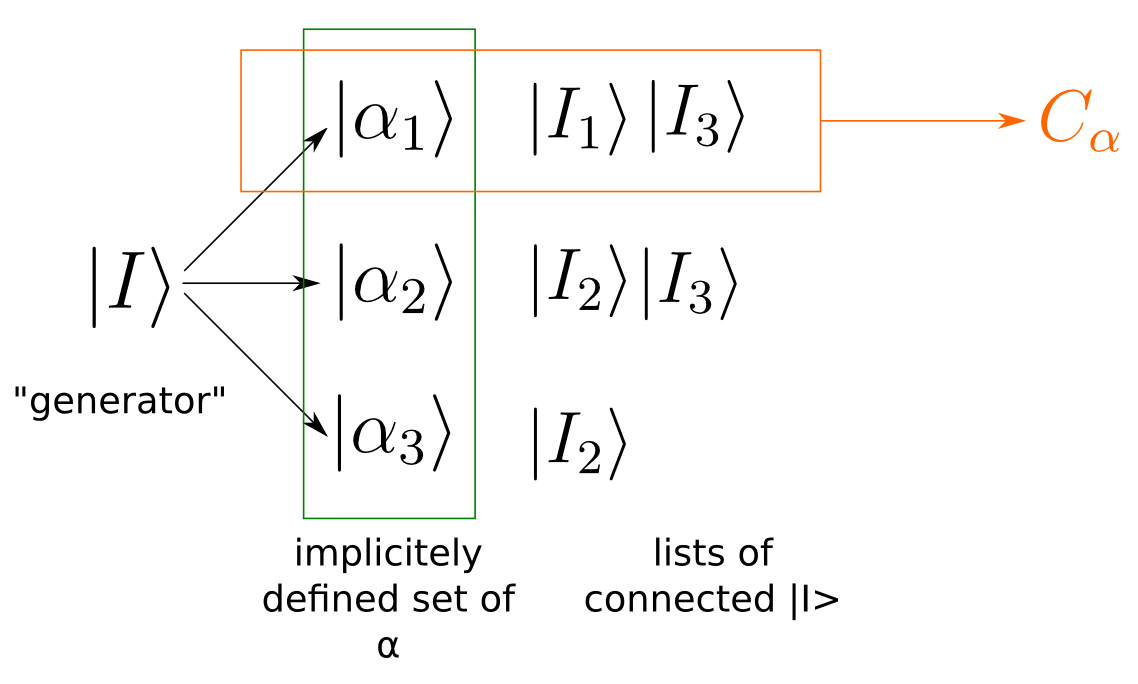
\includegraphics[width=0.7\columnwidth]{figures/matrix_dressing/buildlists}
		\caption{Build lists of connected selectors for unique $\kalpha$'s in batch $G_{pq}$.}
		\label{fig:buildlists}
	\end{center}
\end{figure}

As can be seen, this is very similar to the implementation of CIPSI, except we are building sets instead of incrementing scalars. This, of course, adds complexity to the implementation as the sizes of the $\mathcal{C}_{rs}$ sets aren't known in advance.
%Resizable arrays can be used, although they are not built-in in Fortran.
More importantly, the storage space required may be prohibitive. Noticing that 
\begin{itemize}
\item
all $\Gpqrs$ in a batch are connected to each other,
\item
there are ${\Nvirt}^2$ non-zero $\Gpqrs$ in a batch,
\end{itemize}
and considering a particular case where
\begin{itemize}
\item
$G_{pq}$ is the first batch (all generated $\kalpha$'s are unique)
\item
half of $\Gpqrs$ are internal determinants,
\end{itemize}
we have $\frac{1}{2}{\Nvirt}^2$ unique $\kalpha$'s in the batch each one connecting to at least $\frac{1}{2}{\Nvirt}^2$ internal determinants, for a total storage space of at least $\frac{1}{4}{\Nvirt}^4$.
This case isn't unrealistic, with $\ket {G}$ the Hartree-Fock determinant and $(p,q)$ the highest occupied spinorbitals.

Another issue is the high number of non-contiguous writes in memory, especially with the selectors that connect to all determinants of the batch ; they need to be added to ${\Nvirt}^2$ sets, which is ${\Nvirt}^2$ non-contiguous writes for a single selector.

We can solve the storage issue and mitigate the number of non-contiguous writes, by creating sets of $\kalpha$ that are subsets of several $\mathcal{C}_{rs}$.
Table \ref{tab:systematic_determination} indicates which $\kalpha = \ket {G_{pq}^{rs}}$ of the current batch a selector $\kS$ connects to. In some cases, there are ``wildcard'' indices $X$ and $Y$. Instead of looping over the possible values for those wildcards and adding $\kS$ to all the corresponding $\mathcal{C}_{rs}$ sets, we are going to give wildcard indices the special value $0$ and build intermediate sets $\tilde{\mathcal{C}}_{rs}$. For example, in the case where both $r$ and $s$ are wildcards for a selector $\ket {D_I}$, instead of adding $I$ to all $\mathcal{C}_{rs}$ sets, we will add it to a single set $\tilde{\mathcal{C}}_{00}$. When computation for the batch is completed, $\mathcal{C}_{rs}$ can be evaluated as
\begin{equation}
\mathcal{C}_{rs} \gets \tilde{\mathcal{C}}_{rs} \cup \tilde{\mathcal{C}}_{r0} \cup \tilde{\mathcal{C}}_{s0} \cup \tilde{\mathcal{C}}_{00}
\end{equation}

Among these intermediate sets only $\tilde{\mathcal{C}}_{r0}$ and $\tilde{\mathcal{C}}_{s0}$ may share common elements. Given its frequency, it is important that this computation is efficient. As is sometimes the case, efficiency implies $\mathcal{C}_{rs}$ are not computed individually, but become available inside a loop. An implementation is proposed as algorithm \ref{alg:compute_connected}, which tries to reuse shared $\tilde{\mathcal{C}}_{rs}$ as much as possible.


\clearpage
\section{Alternative definition of excitation amplitudes in multi-reference state-specific coupled cluster}
\label{sec:exp_article}
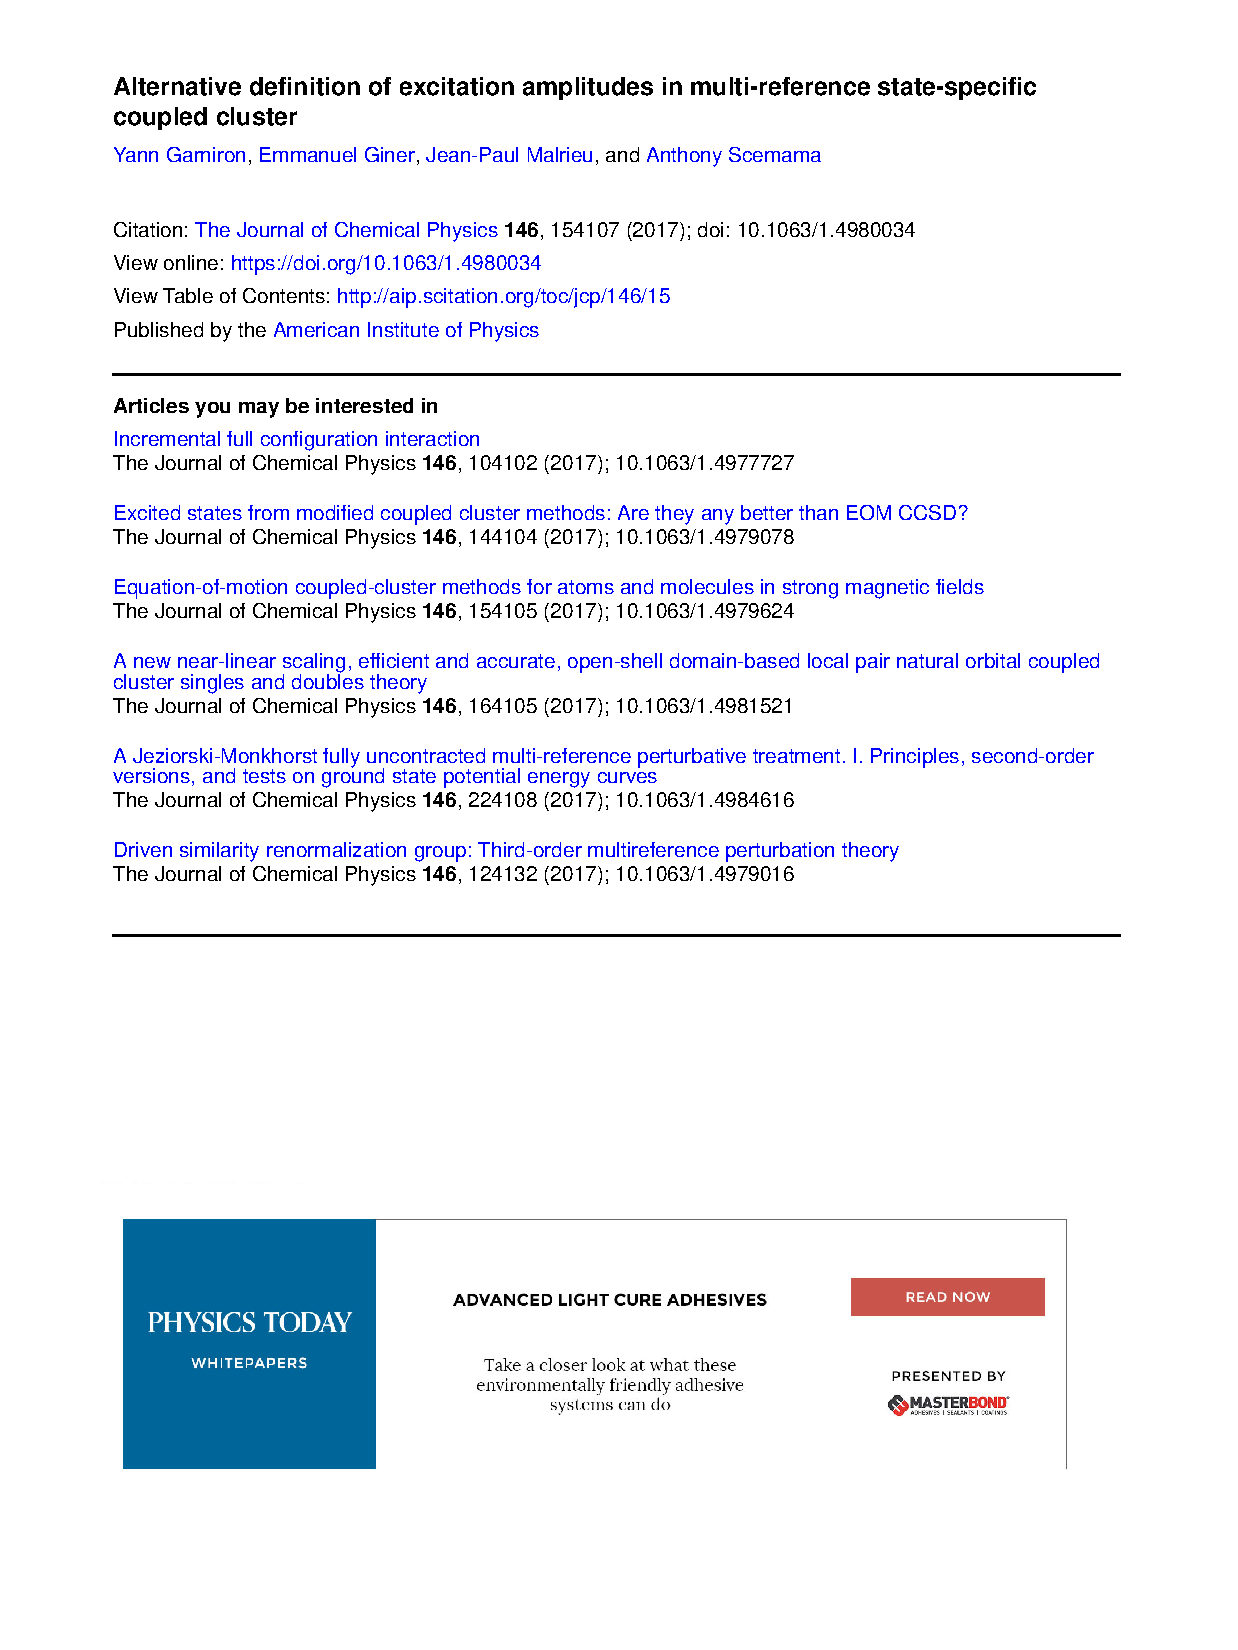
\includepdf[page=2-]{article_mrcc}

\section{Efficient application to Multi-Reference Coupled Cluster}

\newcommand{\interC}[1]{\tilde{\mathcal{C}}_{#1}}
\newcommand{\finC}[1]{\mathcal{C}_{#1}}


\begin{algorithm}
	\caption{Build $\mathcal{C}_{rs}$ from $\tilde{\mathcal{C}}_{rs}$}
	\label{alg:compute_connected}
	\tcc{This takes place after $\tilde{\mathcal{C}}_{rs}$ and $B_{rs}$ for a given batch have been fully computed.}
		\KwData{$\tilde{\mathcal{C}}_{rs}$ the intermediate sets assumed to be sorted with increasing order, $B_{rs}$ the tag matrix}
		%\KwResult{$Z^\star(\Gpqrs, \mathcal{C}_{rs})$ is called for all $\Gpqrs$ of $G_{pq}$ batch that are unique $\kalpha$}
		\KwResult{$\mathcal{C}_{rs}$ is computed for all $\Gpqrs$ of $G_{pq}$ batch that are unique $\kalpha$} 
		\tcc{$\interC{rs}$ and $\finC{rs}$ are considered arrays, the syntax $\finC{rs}[i\ldots j]$ is used to denote a segment of array, $|\finC{rs}|$ is the cardinality of $\finC{rs}$}
		$L$ an array of determinants size $\Nsel$ \;
        $i_1 \gets |\interC{00}|$ \;   
        $L[1 \ldots i_1] \gets \interC{00}[1 \ldots {i_1}]$ \;
        
		\tcc {$B_{r0} = \TRUE$ if column $r$ is entirely tagged}		
		\ForAll{$r ; \neg B_{r0}$}{
		  $i_2 \gets i_1 + |\interC{r0}|$ \;
		  $L[i_1+1 \ldots i_2] \gets \interC{r0}$ \;
		  \ForAll{$s;\neg (B_{rs} \vee B_{0s})$}{
            $i_3 \gets i_2$ \;
            $j \gets 1$ \;
            $k \gets 1$ \;
            \While{$k \leq |\interC{s0}|$}{
              \uIf{$(j > |\interC{r0}|) \vee (\interC{s0}[k] < \interC{r0}[j])$}{
                 $i_3 \gets i_3 + 1$ \;
                 $L[i_3] \gets \interC{s0}[k]$ \;
                 $k \gets k + 1$ \;
              }
              \uElseIf{$\interC{s0}[k] > \interC{r0}[j]$}{
                $j \gets j + 1$ \;
              }
              \Else{
                $j \gets j + 1$ \;
                $k \gets k + 1$ \;
			  }
		    }
		    $i_4 \gets i_3 + |\interC{rs}|$ \;
		    $L[i_3+1 \ldots i_4] \gets \interC{rs}$ \;
		    \tcc{ $L = \finC{rs}$}
		  }
		}
\end{algorithm}



\begin{algorithm}
\caption{Compute a $c_\alpha$ for MR-CC}
\KwData{$\kalpha$ the considered external determinant}
\KwData{$\ket {D_I}$ the list of $N$ internal determinants connected to $\kalpha$, sorted by increasing integer value}
\KwData{$\ket {R_i}$ the list of $\Nref$ reference determinants sorted by increasing integer value and $c_{R_i}$ the associated coefficient}
\KwData{$t_{R_r \rightarrow D_I}$ the used amplitudes}
\KwResult{$c_\alpha$} 

$c_\alpha \gets 0$ \;
Discard $R_r$ when $\text{EXC\_DEGREE} (R_r, \alpha) > 4$ \;
If $R_r$ so that $\text{EXC\_DEGREE} (R_r, \alpha) \leq 2$ was found, discard $\kalpha$ \;


\ForAll{$D_J$}{
\tcc{Note that $\phase{\ket {D_J}}{\kalpha}$ may be pre-computed here}
$\delta \gets \alpha - D_J$ \;
$i \gets 1$ \;
$r \gets 1$ \;
\While{$i \leq N \wedge r \leq N_{ref}$}{
	\uIf{$D_I - R_r > \delta$}{
		$r \gets r + 1$ \;
	}
	\uElseIf{$D_I - R_r < \delta$}{
		$i \gets i + 1$ \;
	}
	\Else
	{
		\If{$R_r \oplus D_I \oplus D_J \oplus \alpha = 0$}{
			\tcc{diamond found}
			$\varphi \gets \phase{\ket {D_J}}{\kalpha} \times \phase{\ket {R_r}}{\ket {D_I}}$ \;
			$c_\alpha \gets c_\alpha + \varphi \times c_{R_r} \times (t_{R_r \rightarrow D_I}) \times (t_{R_r \rightarrow D_J})$ \;
		}
		$r \gets r + 1$ \;
		$i \gets i + 1$ \;
	}
}
}
\end{algorithm}


%\begin{equation}
%incomplet : c_\alpha = \sum_{(\hat p, \hat q, R);\hat p \hat q \ket R = \kalpha} \varphi \times c_R t_p t_q
%\end{equation}

The equation for $c_\alpha$ as well as the procedure for computing amplitudes is detailed in the article presented in section~\ref{sec:exp_article}. In particular, Eq.(26) shows the formula to compute $c_\alpha$ as a sum over what can be described as ``diamond'' structures. 

%\begin{figure}[h!]
	\begin{center}
		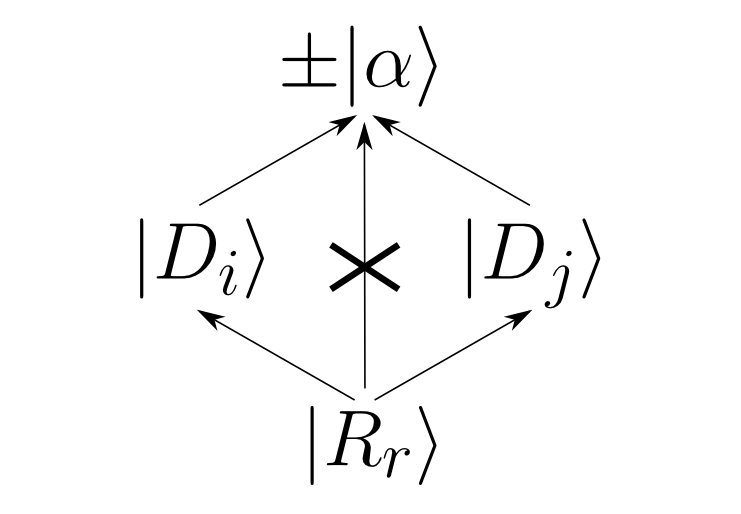
\includegraphics[width=0.3\columnwidth]{figures/matrix_dressing/diamond}
		%\caption{Build lists of connected selectors for unique $\kalpha$ in batch $G_{pq}$}
		%\label{fig:buildlists}
	\end{center}
%\end{figure}

With $\kalpha$ the external determinant being considered, $\ket {D_I}$ and $\ket {D_J}$ internal determinants, and $\ket {R_r}$ a reference determinant.  Parallel arrows indicate connections (excitation degree at most 2) by the same excitation, the vertical arrow indicates $\ket {R_r}$ and $\kalpha$ aren't connected (excitation degree at least 3). More generally, we only consider $\kalpha$ determinants that are not connected to any $\ket {R_r}$. All the determinants we are considering are ordered according to $\ordering$.

The matrix dressing implementation supplies $\{\mathcal{D}\}$ the complete set of the $\Ndet$ internal determinants that connect to $\kalpha$. We call $\{\mathcal{R}\}$ the set of the $\Nref$ reference determinants.

A naive way to find those diamonds, would be to loop over all unordered triplets 
\begin{equation}
(D_I \in \{\mathcal{D}\}, D_J \in \{\mathcal{D}\}, R_r \in \{\mathcal{R}\})
\end{equation}
so that
\begin{equation}
\hat T_{R_r \rightarrow D_I} \hat T_{R_r \rightarrow D_J} \ket {R_r} = \pm \kalpha
\end{equation}
with $\hat T_{R_r \rightarrow D_I}$ the excitation operator so that $\hat T_{R_r \rightarrow D_I} \ket R_r = \kI$.


Using excitation operators, a diamond can be identified by only verifying
\begin{equation}
\hat T_{R_r \rightarrow D_I} = \pm \hat T_{D_J \rightarrow \alpha}
\label{eq:excitation_diamond}
\end{equation}
or in other words, that $\hat T_{R_r \rightarrow D_I}$ and $\hat T_{D_J \rightarrow \alpha}$ involve the same holes and particles.
%(the sign of $\hat T_{D_J \rightarrow \alpha}$ sets the sign in of $\kalpha$ in a diamond).
We first set up a method to identify a diamond, then two methods to ``locate'' them.


\paragraph{Identifying diamonds}
For implementational efficiency, we are going to express excitations using $\hat f_p$ an operator that flips the occupation status of a spinorbital $p$.
\begin{align}
  \begin{cases}
  \hat f_p \ket A = \ordering a_p \ket A & \text{if }  a_p \ket A \neq 0\\
  \hat f_p \ket A = \ordering a^\dagger_p \ket A & \text{if }  a^\dagger_p  \ket A \neq 0\\
  \end{cases}
\end{align}
or in a less verbose formulation
\begin{equation}
\hat f_p = \ordering a_p + \ordering a^\dagger_p
\end{equation}
This avoids the burden of making a distinction between annihilation and creation operator, and of checking whether they can be applied to a determinant. This also ignores phase factors.


The notation $\hat f_{ab\ldots}$ will be used as a shortcut for $\hat f_a \hat f_b \ldots$, and we define $\hat F_{A \rightarrow B} = \hat F_{B \rightarrow A}$ as the set of $\hat f$ operators that flips all spinorbitals whose occupation differ between $\ket A$ and $\ket B$.

Clearly a set of $\hat f$ operators does not univocally correspond to an excitation, but it is demonstrable that in this particular case, we can use $\hat F$ instead of the excitation operator $\hat T$, i.e. we can ensure $(R_r, D_I, D_J, \alpha)$ are forming a diamond by only verifying
\begin{equation}
\hat F_{R_r \rightarrow D_I} = \hat F_{D_J \rightarrow \alpha}
\label{eq:diamond_flip}
\end{equation}

It is easy to understand from Eq.~\eqref{eq:excitation_diamond} how this is a necessary condition, it is less obvious that it is also a sufficient one, i.e. that this can only happen if there is a diamond. In fact, it is not generally true. It is demonstrable in this particular case thanks to the known excitation degrees. It is known $\ket {D_I}$ and $\ket {D_J}$ are connected by at most a double excitation to $\kalpha$, therefore at most 4 orbitals have their occupation status flipping, two of them occupied and two unoccupied in $\kalpha$. For later clarity we use the dot ($\dot a$) notation to denote indices of spinorbitals that are occupied in $\kalpha$.

\begin{equation}
\hat F_{D_I \rightarrow \alpha} = \hat F_{R_r \rightarrow D_J} = \hat f_{\dot a \dot bcd} \; ; \; \hat F_{D_J \rightarrow \alpha} = \hat F_{R_r \rightarrow D_I} = \hat f_{\dot e \dot fgh}
\end{equation}

The reference determinant $\ket {R_r}$ is reached from $\kalpha$ after chaining the two ``flippings''.

\begin{equation}
\hat F_{R \rightarrow \alpha} = (\hat f_{\dot a \dot bcd})(\hat f_{\dot e \dot fgh})
\end{equation}

If indices $\dot a,\dot b,c,d,\dot e,\dot f,g,h$ are all unique, $\hat T_{R \rightarrow D_I}$ and $\hat T_{D_J \rightarrow \alpha}$ are independent and thus can be chained, so the diamond is valid. If they are not, the diamond is still known to be valid thanks to our knowledge that $\kalpha$ is at least a triple excitation from $\ket {R_r}$, and therefore at least 6 orbitals must flip. 

It is trivial that

\begin{equation}
\hat f_{aa} = \hat 1
\end{equation}

so only 2 among the 8 indices can refer to the same spinorbital $x$ (which we arbitrarily choose unoccupied in $\kalpha$). For obvious reasons one is found among $(\dot a,\dot b,c,d)$ and the other among $(\dot e,\dot f,g,h)$.

\begin{equation}
\hat F_{R \rightarrow \alpha} = (\hat f_{\dot a \dot bcx})(\hat f_{\dot e \dot fgx}) = (\hat f_{\dot a \dot bc})(\hat f_{\dot e \dot fg})
\end{equation}

As can be seen, applying $(\hat f_{\dot a \dot bc})(\hat f_{\dot e \dot fg})$ to $\kalpha$ will flip four occupied spinorbitals versus only two unoccupied ones ; this implies $\kalpha$ has two extra electrons compared to $\ket {R_r}$. Because we know this not to be the case, we know such a situation cannot happen.

Now that we know Eq.~\eqref{eq:diamond_flip} is sufficient to identify a diamond, we have to write its implementational expression, which is straightforward. The set of spinorbitals whose occupation status differ between $\ket A$ and $\ket B$ can be computed as a bitstring as
\begin{equation}
A \oplus B
\end{equation}
with $A$ a single bitstring associated with $\ket A$ ---~the association between a spinorbital and a bit is arbitrary.

Eq.~\eqref{eq:diamond_flip} is verified iff
\begin{equation}
R_r \oplus D_I = D_J \oplus \alpha
\end{equation}
or alternatively, since $A \oplus A = 0$
\begin{equation}
R_r \oplus D_I \oplus D_J \oplus \alpha = 0
\label{eq:diamond_xor}
\end{equation}

\paragraph{Locating diamonds by binary search}
Now that we expressed the identification of a diamond in a simple way, we must figure a strategy to find them fast. Eq.~\eqref{eq:diamond_xor} can be rewritten as
\begin{equation}
D_J = R_r \oplus D_I \oplus \alpha
\end{equation}
which implies a simple algorithm that finds the diamonds in $\mathcal{O}(N \times \Nref \times \log(N))$:
\begin{enumerate}
\item
Iterate over $(R_r, D_I)$
\item
Binary search for $D_J = (R_r \oplus D_I \oplus \alpha)$ in $\{\mathcal{D}\}$ if $||D_J|| = \Nelec$.
\end{enumerate}

Depending on the sizes of the $\{D\}$ and $\{R\}$ sets, an alternative variant can also be used, giving a complexity of $\mathcal{O}(N^2 \times \log(\Nref))$:
\begin{enumerate}
\item
iterate over $(D_I, D_J)$
\item
binary search for $R_r = (D_I \oplus D_J \oplus \alpha)$ in $\{\mathcal{R}\}$ if $||R_r|| = \Nelec$.
\end{enumerate}

Those are desirable if one of $\{\mathcal{D}\}$ or $\{\mathcal{R}\}$ is relatively small, in particular, in case of single-reference computation, i.e. $|\mathcal{R}|=1$, the former variant is ideal. For larger sets, however, a more complex variant with a complexity $\mathcal{O}(N \times (N+\Nref))$ is introduced next.


\paragraph{Locating diamonds by rewriting excitations as additions}
Although the method could be chosen on a ``by-$\alpha$'' basis depending on $N$ and $\Nref$, only this one is currently used in the \QP as it works for larger sets.
Unlike the previous one, this method may yield false positives, thus it uses Eq.~\eqref{eq:diamond_xor} for confirmation.
The idea is to express an excitation as an addition. As was said, bitstrings can be interpreted as integers, so they can be added, subtracted and compared as such. As in the case of the $\hat f$ operator, this approach entirely ignores phase factors. We can easily associate the integer values $T_{A \rightarrow B}$ and $T_p^q$ to excitations $\pm \hat T_{A \rightarrow B}$ and $\pm \hat T_p^q$ respectively.
\begin{align}
T_p^q & = 2^{q-1} - 2^{p-1} \\
T_{A \rightarrow B} & =  B - A \\
T_{A \rightarrow B} + A & = B 
\end{align}
With $A$ the bitstring associated with $\ket A$ as a single integer ---~the association between a spinorbital and a bit is arbitrary. It is a necessary but not sufficient condition for a diamond that
\begin{equation}
T_{R \rightarrow D_I} = T_{D_J \rightarrow \alpha}
\end{equation}
Indeed,
\begin{align}
\pm \hat T \ket A = \ket B \implies  T + A = B\\
T + A = B \centernot \implies \pm \hat T \ket A = \ket B
\end{align}
with $T$ the integer associated with excitation $\pm \hat T$. If $\pm \hat T \ket A = 0$, in most cases $T + A$ will yield a bitstring with a wrong number of bits/electrons, but this is not guaranteed, hence the rare presence of false positives.

Eq.~\eqref{eq:excitation_diamond} implies
\begin{equation}
D_I - R_r = \alpha - D_J 
\end{equation}
Finding all $(D_I, R_r)$ pairs that verify this, assuming $\{\mathcal{D}\}$ and $\{\mathcal{R}\}$ are sorted in ascending order, can be achieved with linear complexity.

% with a complexity of either $\mathcal{O}(N + N_{ref})$ or $\mathcal{O}(N \times min(N, N_{ref}) \times log(max(N, N_{ref})))$

\begin{enumerate}
\item
Initialize $I$ and $r$ to $1$
\item
Loop while both $I$ and $r$ are not out of bounds
\item
If $D_I - R_r < \alpha - D_J$, increment $I$ and loop
\item
If $D_I - R_r > \alpha - D_J$, increment $r$ and loop
\item
If $D_I - R_r = \alpha - D_J$, a $(D_I, R_r)$ pair has been found. Check if a diamond can be formed using Eq.~\eqref{eq:diamond_xor}. Increment $I$ and $r$, and loop.
\end{enumerate}
The complexity is $\mathcal{O}(N \times (N+\Nref))$.

For implementational ease and efficiency, two things are worth noting:
\begin{itemize}

\item
Integer overflows do not need to be handled. The size of integers being limited to 64 bits essentially means an unsigned integer $I$ is represented as $I \mod{2^{64}}$. Quite fortunately modulus has the properties of compatibility with addition and substraction.
\begin{align}
a_1 + a_2 &\equiv b_1 + b_2 \mod{n} \\
a_1 - a_2 &\equiv b_1 - b_2 \mod{n}
\end{align}
with $a_1 \equiv b_1 \mod n$, and $a_2 \equiv b_2 \mod n$. When it comes to addition and substraction, signed and unsigned integers are equivalent, so signed integers can be used as well.
\item
It is not required to handle bitstrings as actual arbitrary size integers when it comes to addition and subtraction. While addition to a bitstring was introduced as being associated with an excitation, it can actually be associated with any combination of creation and annihilation operators. It is therefore valid to consider each 64-bit integer as an independent ``sub-bitstring'' on which a subset of the operators will be applied. In short, additions and subtractions can be done integer-wise, without the overhead of handling carries.
\end{itemize}
When it comes to comparison, since the 64 bit integers corresponding to the lower orbitals will typically have more mobile electrons, they should be given them more weight to resolve comparison as fast as possible.

\paragraph{Computing the phase factor}



So far we have ignored phase factors, but we need to know the sign of $\kalpha$ in each found diamond. This can be tricky, since confusion can easily arise from reference-dependent and reference-independent notations. To keep generality, we use reference-dependent notations, unlike Eq.~(26) of the presented article.

Assuming
\begin{equation}
\hat T_{pq}^{rs} \ket I = \pm \ket i
\end{equation}
reference-independent notation for amplitude $t_{pq \rightarrow rs}$ and reference-dependent notation $t_{I \rightarrow i}$ could be wrongfully assumed equivalent. This is not the case, since $t_{pq \rightarrow rs}$ is associated with excitation $\hat T_{pq}^{rs}$ as described in chapter \ref{chap:DET_DRIVEN} ---~with a particular ordering for creation an annihilation operators~--- while $t_{I \rightarrow i}$ is associated with $\hat T_{I \rightarrow i}$ so that
\begin{equation}
\hat T_{I \rightarrow i}  \ket I = \ket i
\end{equation}
preserving the phase factor of $\ket i$. Therefore
\begin{equation}
t_{I \rightarrow i} = \frac{t_{pq \rightarrow rs}}{\phase{\ket I}{\ket i}}
\end{equation}

In order to compute the contribution of a diamond to $c_\alpha$, we are required to compute the phase factor
\begin{equation}
\phase{\ket {R_r}}{\kalpha} = \phase{\ket {R_r}}{\ket {D_I}}\, \phase{\ket {D_I}}{\kalpha}
\end{equation}
which is noted $(-1)^{n(I \rightarrow \alpha)}$ in Eq.~(26) of the presented article, with $I$ the reference determinant. The article uses the reference-independent notation for amplitudes. If we re-write the formula with reference-dependent notations, the contribution for each diamond becomes
\begin{equation}
c_r \phase{\ket {R_r}}{\kalpha} \frac{t_{R_r \rightarrow D_I}}{\phase{\ket {R_r}}{\ket {D_I}}} \frac{t_{D_I \rightarrow \alpha}}{\phase{\ket {D_I}}{\kalpha}} =c_r t_{R_r \rightarrow D_I} t_{D_I \rightarrow \alpha}
\end{equation}
with $c_r$ the coefficient of $\ket {R_r}$.
The amplitudes for $t_{D_I \rightarrow \alpha}$ of course cannot be stored and would be too expensive to compute on the fly. Because $\hat T_{D_I \rightarrow \alpha}$ involves the same orbitals as $\hat T_{R_r \rightarrow D_J}$, their associated amplitudes are the same up to the phase factor
\begin{equation}
t_{D_I \rightarrow \alpha} = t_{R_r \rightarrow D_J} \phase{\ket {R_r}}{\ket {D_J}} \, \phase{\ket {D_I}}{\kalpha}
\end{equation}
So we can finally rewrite the contribution to $c_\alpha$ for each diamond
\begin{equation}
c_r t_{R_r \rightarrow D_I} t_{R_r \rightarrow D_J} \phase{\ket {R_r}}{\ket {D_J}}\,\phase{\ket {D_I}}{\kalpha}
\end{equation}

\end{document}
